\section{Method}

\subsection{Problem Formulation}
Let $\mathcal D_L=\{(X_i,Y_i)\}$ and $\mathcal D_U=\{X_j\}$ denote labeled and unlabeled MRI volumes. A student $f_\theta$ is optimized by gradient descent, while a teacher $f_\xi$ is updated as
\begin{equation}
\xi \leftarrow \alpha\xi+(1-\alpha)\theta.
\end{equation}
Both networks use the same 2D U-Net architecture. During training only, a center slice $z$ is accompanied by its immediate neighbors $z-1$ and $z+1$. Inference uses only the native center slice.

\subsection{Paired Through-Plane Observation}
We parameterize a three-tap virtual slice profile by width $\sigma$ and phase $\phi$:
\begin{equation}
w_k(\sigma,\phi)=
\frac{\exp\!\left[-(k-\phi)^2/(2\sigma^2)\right]}
{\sum_{j=-1}^{1}\exp\!\left[-(j-\phi)^2/(2\sigma^2)\right]},
\quad k\in\{-1,0,1\}.
\label{eq:profile}
\end{equation}
The weights are nonnegative and sum to one. We use the bounded support $\sigma\in[0.45,0.85]$ and $\phi\in[-0.25,0.25]$ inherited by the frozen development protocol. For a stack $V_z=(v_{z-1},v_z,v_{z+1})$, define
\begin{equation}
\mathcal A_w(V_z)=\sum_{k=-1}^{1}w_kv_{z+k}.
\label{eq:operator}
\end{equation}
All pixels in a sample share the same $w$; this is a slice-level observation, not pixelwise MixUp.

The key rule is to apply $\mathcal A_w$ to both members of a training pair. For labeled data,
\begin{equation}
\widetilde x_z^L=\mathcal A_w(X_z^L),\qquad
q_z^L=\mathcal A_w\!\left(\operatorname{onehot}(Y_z^L)\right).
\label{eq:labeled_pair}
\end{equation}
For unlabeled data, the teacher first predicts and post-processes each neighboring slice with the inherited two-dimensional largest-connected-component rule:
\begin{equation}
\widehat y_{z+k}^U=\operatorname{LCC}
\left(\arg\max f_\xi(x_{z+k}^U)\right).
\end{equation}
The corresponding pair is
\begin{equation}
\widetilde x_z^U=\mathcal A_w(X_z^U),\qquad
q_z^U=\mathcal A_w\!\left(\operatorname{onehot}(\widehat Y_z^U)\right).
\label{eq:unlabeled_pair}
\end{equation}
Thus $q_{z,c}(v)\in[0,1]$ and $\sum_cq_{z,c}(v)=1$. It is exact with respect to the discrete labels and chosen operator, but it is not claimed to be the unknown continuous physical tissue fraction.

\subsection{Moment-Constrained Profile Design}
Uniform sampling over $(\sigma,\phi)$ is a plausible parent law $p_0$, but it does not account for heterogeneous axial-transition opportunities. We discretize the fixed support of Eq.~\eqref{eq:profile} into a $21\times21$ grid $\{w_g\}_{g=1}^{G}$ and design one global distribution $q\in\Delta^{G-1}$ using labeled training stacks only.

For each labeled patient and normalized axial third, let $s$ denote a stratum and $\mathcal B_s$ the pixels where neighboring hard labels differ. We compute semantic-preserving occupancy entropy
\begin{equation}
u_{s,g}=\frac{1}{|\mathcal B_s|}
\sum_{v\in\mathcal B_s}
H(q_{g,v})
\mathbf 1\!\left[\arg\max q_{g,v}=y_{z,v}\right],
\label{eq:utility}
\end{equation}
where $q_{g,v}$ is the fractional occupancy induced by candidate $g$. The indicator excludes candidates that reverse the center-slice hard semantic at $v$; the entropy rewards non-degenerate fractional information on genuine axial transitions.

The first stage maximizes worst-stratum utility:
\begin{equation}
t^*=\max_{q\in\mathcal Q}\min_s\sum_{g=1}^{G}q_gu_{s,g}.
\label{eq:stage1}
\end{equation}
The feasible set $\mathcal Q$ enforces phase-mirror symmetry and preserves the parent distribution's neighbor mass, squared neighbor mass, and directional moment within a fixed trust region. It additionally bounds each labeled patient--stratum image residual, caps $q_g/p_{0,g}$, and prevents entropy collapse. These constraints prevent Eq.~\eqref{eq:stage1} from gaining utility merely by increasing perturbation strength or concentrating on a few grid points.

The second stage chooses the least-disruptive distribution that retains $99\%$ of the robust optimum:
\begin{equation}
q^*=\arg\min_{q\in\mathcal Q}D_{\mathrm{KL}}(q\|p_0)
\quad\text{s.t.}\quad
\min_s\sum_gq_gu_{s,g}\ge0.99t^*.
\label{eq:stage2}
\end{equation}
The solved $q^*$ is frozen before network training. It is global and patient-independent at run time; it does not access unlabeled labels, validation/test data, predictions, confidence, or losses.

\subsection{Learning Objective and Inference}
After forming the paired unlabeled target, we apply a fixed coordinate-preserving appearance perturbation $G_\eta$ only to $\widetilde x_z^U$:
\begin{equation}
(X^U,\widehat Y^U)\xrightarrow{\mathcal A_w}
(\widetilde x_z^U,q_z^U)\xrightarrow{G_\eta}
(G_\eta(\widetilde x_z^U),q_z^U).
\end{equation}
The target-changing observation is therefore paired before any target-preserving appearance variation. We use the same fixed appearance policy in all matched experiments; it is a training regularizer rather than an additional methodological component.

Let $p=\operatorname{softmax}(f_\theta(x))$. For a fractional target $q$, we use soft cross-entropy and soft Dice:
\begin{align}
\mathcal L_{\mathrm{SCE}}(p,q)&=-\frac{1}{|\Omega|}
\sum_{v,c}q_{v,c}\log p_{v,c},\\
\mathcal L_{\mathrm{SD}}(p,q)&=\frac{1}{C}\sum_c
\left(1-\frac{2\sum_vp_{v,c}q_{v,c}+\epsilon}
{\sum_vp_{v,c}^2+\sum_vq_{v,c}^2+\epsilon}\right),\\
\mathcal L_{\mathrm{occ}}&=\tfrac12
(\mathcal L_{\mathrm{SCE}}+\mathcal L_{\mathrm{SD}}).
\end{align}
After the inherited 1,000-iteration supervised warm-up, each loader batch contains 12 labeled and 12 unlabeled center slices and yields 36 student views: 12 native labeled, 12 paired re-acquired labeled, and 12 paired re-acquired unlabeled. The complete objective is
\begin{equation}
\mathcal L=
\tfrac12\left[
\mathcal L_{\mathrm{hard}}(f_\theta(x_z^L),y_z^L)+
\mathcal L_{\mathrm{occ}}(f_\theta(\widetilde x_z^L),q_z^L)
\right]
+\lambda(t)\mathcal L_{\mathrm{occ}}
\left(f_\theta(G_\eta(\widetilde x_z^U)),q_z^U\right).
\label{eq:full_loss}
\end{equation}
The teacher receives EMA updates and no gradient. At inference,
\begin{equation}
\widehat y_z=\arg\max f_\theta(x_z),
\end{equation}
so neighboring slices, profile design, teacher prediction, and appearance perturbation are all removed.

\begin{figure*}[t]
    \centering
    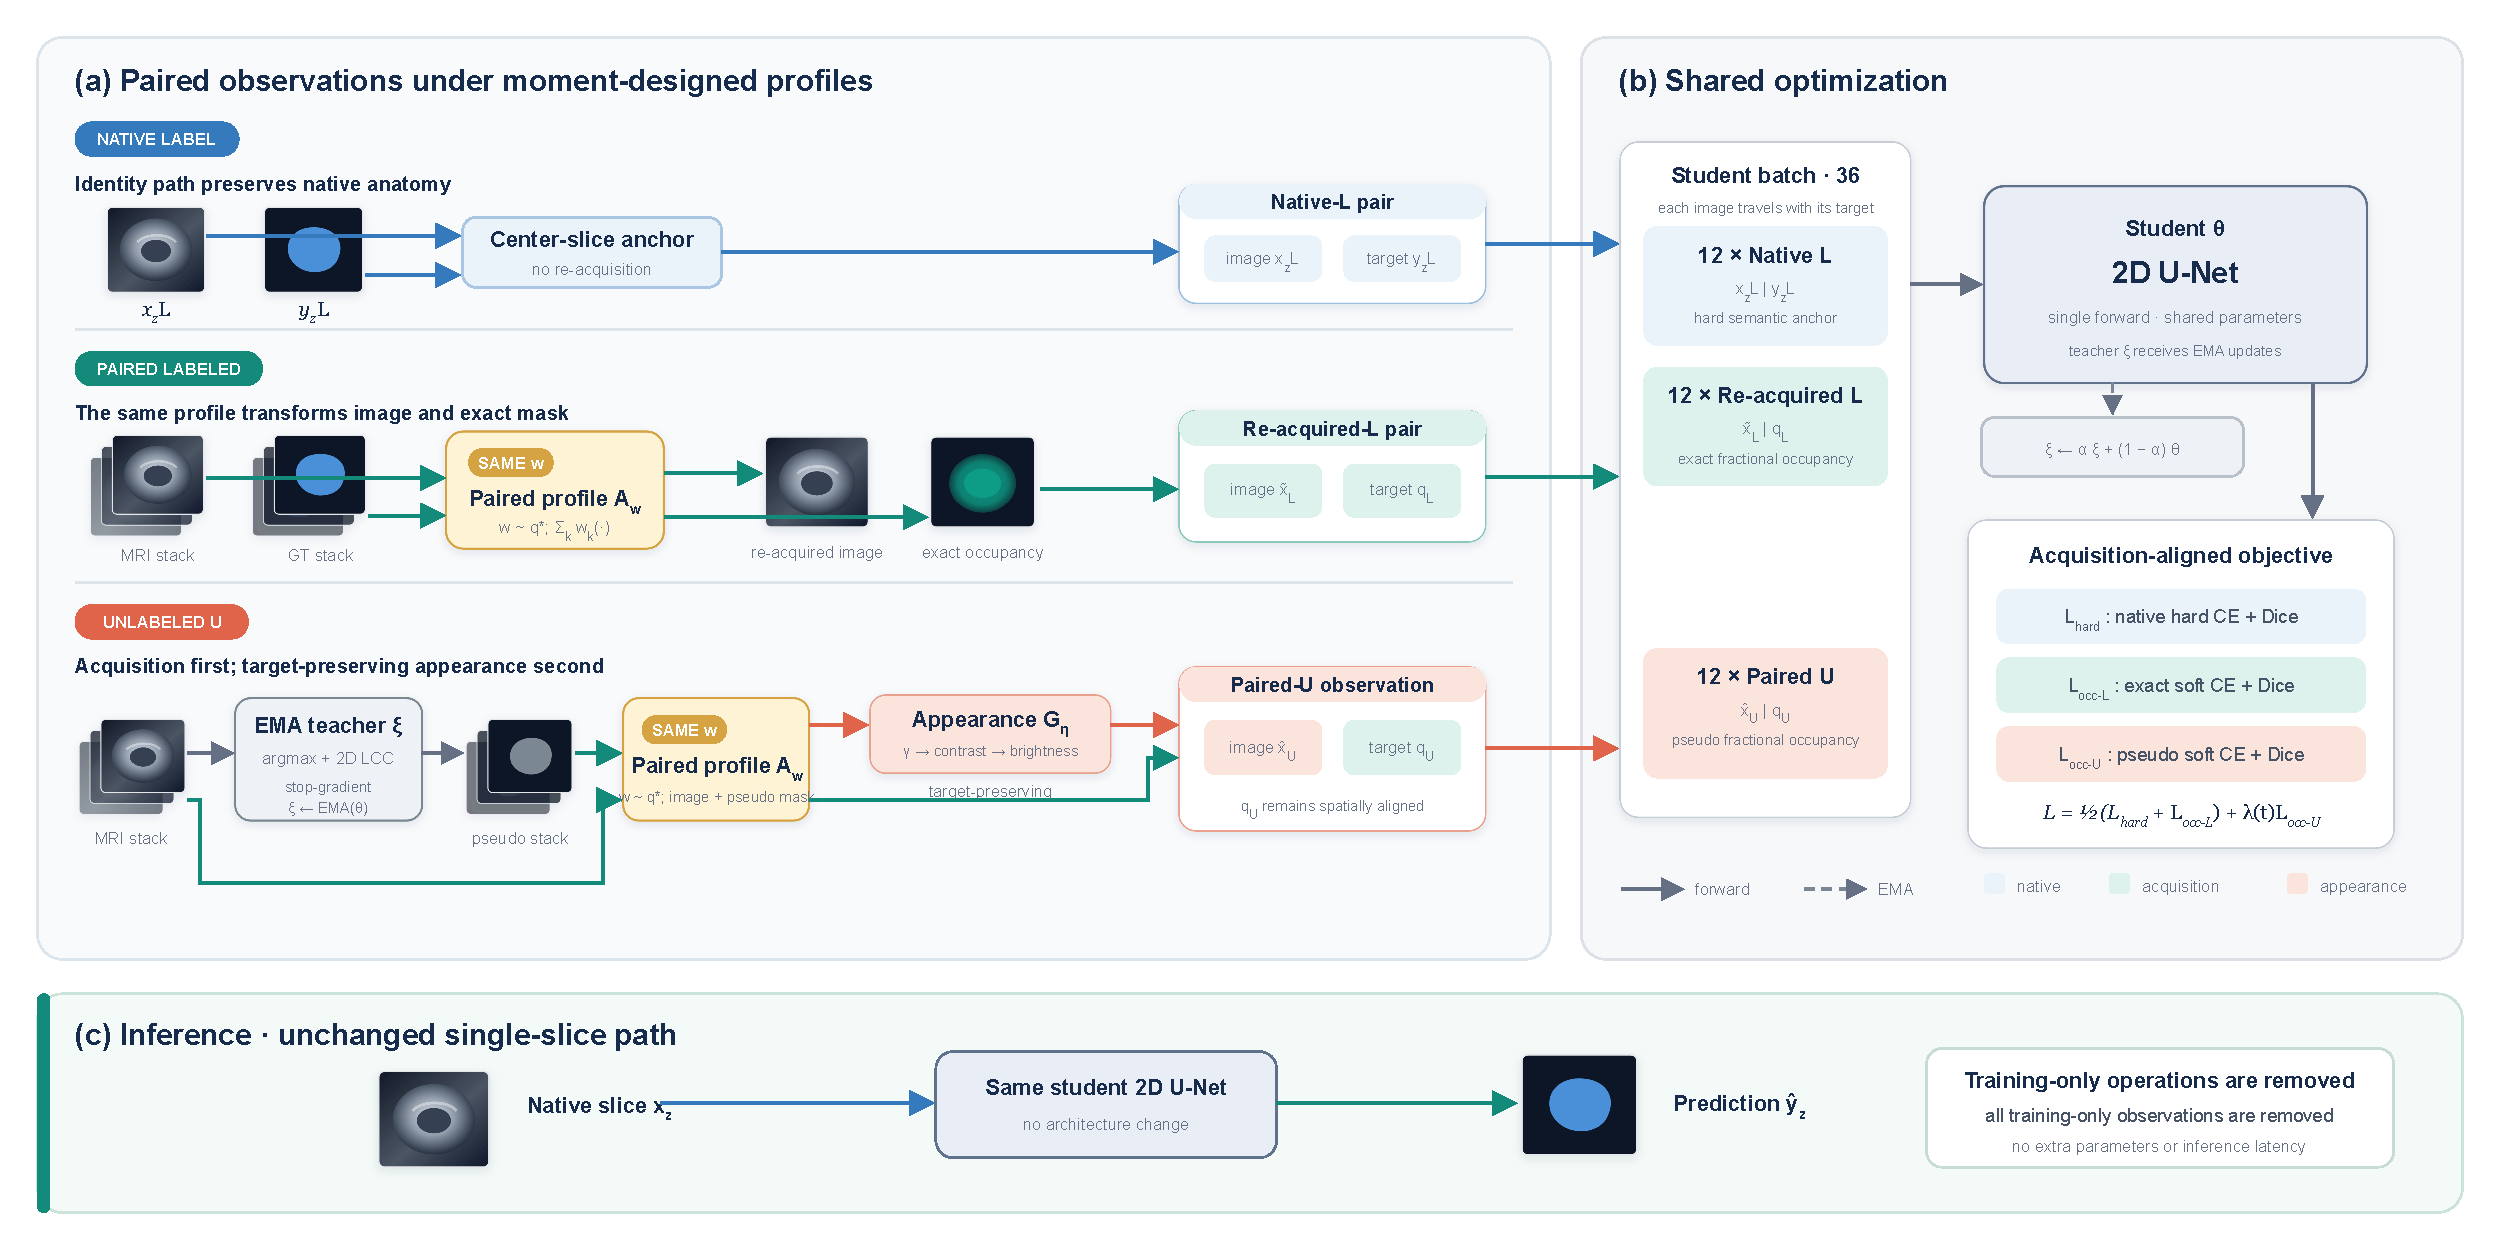
\includegraphics[width=\textwidth]{fig/method_pipeline.pdf}
    \caption{Overview of \method. Native labeled samples provide a hard semantic anchor, while labeled and unlabeled neighboring slices are transformed into paired image--occupancy observations by the same sampled profile. A single student is optimized from all views and updates the EMA teacher. The profile law is designed once from labeled training data, and inference remains an unchanged single-slice 2D path.}
    \label{fig:method}
\end{figure*}
